\documentclass[aspectratio=169]{beamer}
\graphicspath{ {./images/}}

\title{CP Rate My Professor}
\usetheme[]{Berlin}
\setbeamertemplate{navigation symbols}{}
\makeatletter
  \setbeamertemplate{footline}{%
    \begin{beamercolorbox}[colsep=1.5pt]{upper separation line foot}
    \end{beamercolorbox}
    \begin{beamercolorbox}[ht=2.5ex,dp=1.125ex,%
      leftskip=.3cm,rightskip=.3cm plus1fil]{author in head/foot}%
      \leavevmode{\usebeamerfont{author in head/foot}\insertshortauthor}%
      \hfill%
      {\usebeamerfont{institute in head/foot}\usebeamercolor[fg]{institute in head/foot}\insertshortinstitute}%
    \end{beamercolorbox}%
    \begin{beamercolorbox}[ht=2.5ex,dp=1.125ex,%
      leftskip=.3cm,rightskip=.3cm plus1fil]{title in head/foot}%
      {\usebeamerfont{title in head/foot}\insertshorttitle\hfill\insertframenumber}%
    \end{beamercolorbox}%
    \begin{beamercolorbox}[colsep=1.5pt]{lower separation line foot}
    \end{beamercolorbox}
  }
\makeatletter

\begin{document}
\frame{\titlepage}
\begin{frame}
    \frametitle{Online Learning}
    \begin{itemize}
        \item We've been at home for more than two years now
    \end{itemize}
\end{frame}
\begin{frame}

\end{frame}
\begin{frame}
    \frametitle{A sad, true story}
    \pause
    \begin{columns}
        \begin{column}{0.4\textwidth}
            \centering
            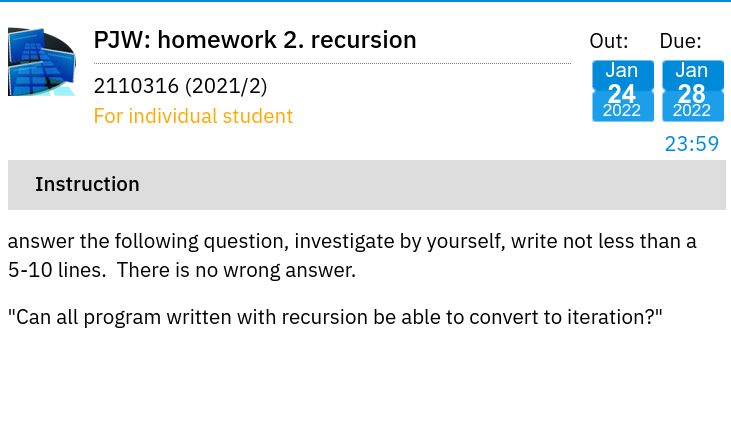
\includegraphics[scale=0.3]{proglangsec1}
            
\includegraphics[scale=0.5]{proglangsec1_nowrong}
        \end{column}
        \pause
        \begin{column}{0.4\textwidth}
            \centering
            
\includegraphics[scale=0.2]{proglangsec2}
        \end{column}
    \end{columns}
\end{frame}
\begin{frame}
    \centering
    {\huge \textbf{Meet CP Rate My Professor!}}
\end{frame}
\begin{frame}
    \frametitle{CP Rate My Professor}
    \begin{itemize}
        \pause
        \item CP Rate My Professor is a platform for commenting and rating professor\pause
        \item Our number one goals is \underline{\textbf{transparency}} and \underline{\textbf{anonymity}} for the person giving the comments
    \end{itemize}
\end{frame}
\begin{frame}
    \frametitle{Our application}
    \begin{center}
    \begin{columns}
        \begin{column}{0.3\textwidth}
            \centering
            -- Home Page --
        \end{column}
        \begin{column}{0.3\textwidth}
            \centering
            -- Professor Page --

        \end{column}
        \centering
        -- New Comment Page --
        \begin{column}{0.3\textwidth}

        \end{column}
    \end{columns}
    \end{center}
\end{frame}
\end{document}
